\chapter{Testarea aplicației și rezultate experimentale}
\label{cap:cap4}

Acest capitol detaliază procesul de validare practică a platformei propuse. Având în vedere natura IaaS a aplicației, a cărei utilitate depinde direct de integrarea cu mediul fizic, evaluarea nu se limitează la teste unitare izolate. Este verificată funcționarea sistemului în ansamblu, desfășurat pe un cluster OpenStack operațional. Inițial, sunt descrise topologia mediului de testare și procedura de inițializare, urmate de strategia de evaluare și gradul de acoperire a cerințelor. În secțiunea finală, sunt analizate rezultatele care atestă execuția corectă a operațiunilor fundamentale: provizionarea instanțelor virtuale, injectarea cheilor SSH și accesul la consola grafică prin noVNC.

\section{Mediul de testare}
\label{sec:cap4_mediu}

Platforma a fost testată într-un mediu de tip \textit{private cloud}, construit pe o singură mașină fizică. Pe stația gazdă (sistem de operare Windows~11) rulează atât hipervizorul VMware, care găzduiește mașina virtuală cu OpenStack, cât și stiva de servicii de management (API-ul FastAPI, procesele Celery și interfața Nuxt). Comunicarea dintre stația de dezvoltare și API-ul OpenStack se realizează printr-un tunel Tailscale, care rutează adresa internă a cluster-ului (\texttt{192.168.144.200/32}), permițând accesul securizat de la distanță. Configurația hardware este prezentată în Tabelul~\ref{tab:cap4_hardware}, iar componentele software și versiunile acestora în Tabelul~\ref{tab:cap4_software}.

\begin{table}[H]
    \centering
    \caption{Configurația hardware a mediului de testare}
    \label{tab:cap4_hardware}
    \begin{tabular}{l l l}
        \hline
        \textbf{Sistem} & \textbf{Rol} & \textbf{Specificații} \\
        \hline
        VM OpenStack & Cluster all-in-one & 8 vCPU, \\
        (Ubuntu Server) & (Kolla-Ansible) & 16 GB RAM, 200 GB disc \\
        \hline
    \end{tabular}
\end{table}


\begin{table}[H]
    \centering
    \caption{Componentele software și versiunile utilizate}
    \label{tab:cap4_software}
    \begin{tabular}{l l l}
        \hline
        \textbf{Categorie} & \textbf{Componentă} & \textbf{Versiune} \\
        \hline
        \multirow{4}{*}{Infrastructură} & OpenStack (release) & 2025.2 (Flamingo) \\
                                        & Kolla-Ansible & 22.1.0 \\
                                        & Ubuntu Server & 24.04.4 LTS \\
                                        & Docker Engine & 4.79.0 \\
        \hline
        \multirow{6}{*}{Backend} & FastAPI & 0.136.3 \\
                                 & Uvicorn & 0.48.0 \\
                                 & Celery & 5.6.3 \\
                                 & SQLAlchemy & 2.0.50 \\
                                 & OpenStack SDK & 4.13.0 \\
                                 & Pydantic & 2.13.4 \\
        \hline
        \multirow{4}{*}{Frontend} & Nuxt & 4.3.1 \\
                                  & Vue & 3.5.28 \\
                                  & Pinia & 3.0.4 \\
                                  & Tailwind CSS (modul Nuxt) & 6.14.0 \\
        \hline
        \multirow{3}{*}{Date și mesagerie} & MariaDB & 11.x \\
                                           & RabbitMQ & 3 (management) \\
                                           & InfluxDB & 2 \\
        \hline
    \end{tabular}
\end{table}

\section{Lansarea platformei}
\label{sec:cap4_punere}

Implementarea practică a platformei necesită configurarea a două componente majore: instanțierea infrastructurii OpenStack (mediul fizic de virtualizare creat cu ajutorul Kolla-Ansible) și activarea aplicațiilor de management ce deservesc logica de business.

\subsection{Desfășurarea infrastructurii OpenStack prin Kolla-Ansible}
\label{subsec:cap4_kolla}

Instalarea manuală a componentelor OpenStack este un proces complicat și predispus la erori. Din acest motiv, infrastructura a fost desfășurată cu \textbf{Kolla-Ansible}, care împachetează fiecare serviciu OpenStack într-un container Docker și automatizează configurarea prin \textit{playbook}-uri Ansible. S-a optat pentru topologia \textit{all-in-one}, în care planul de control și planul de calcul coexistă pe un singur nod. Configurarea este prezentată în fișierul \texttt{globals.yml}:

\begin{lstlisting}[basicstyle=\ttfamily\footnotesize,breaklines=true,frame=single]
# /etc/kolla/globals.yml (optiuni esentiale)
kolla_base_distro: "ubuntu"
openstack_release: "2024.1"
kolla_internal_vip_address: "192.168.144.200"
network_interface: "ens33"            # interfata de management
neutron_external_interface: "ens34"   # interfata pentru reteaua externa
enable_cinder: "yes"
enable_cinder_backend_lvm: "yes"
\end{lstlisting}

\noindent Activarea Cinder cu backend LVM presupune un grup de volume \texttt{cinder-volumes}, creat într-un mediu de dezvoltare pe un fișier de tip \textit{loopback}.

\begin{lstlisting}[basicstyle=\ttfamily\footnotesize,breaklines=true,frame=single]
kolla-genpwd
kolla-ansible bootstrap-servers -i ./all-in-one
kolla-ansible prechecks       -i ./all-in-one
kolla-ansible deploy          -i ./all-in-one
kolla-ansible post-deploy
\end{lstlisting}

\noindent Pasul \texttt{post-deploy} generează fișierul \texttt{admin-openrc.sh}. După încărcarea acestuia, se creează resursele pe care platforma le presupune existente: rețeaua externă din care se alocă adresele IP flotante (variabila \texttt{OS\_EXTERNAL\_NETWORK}) și imaginile de bază (\texttt{cirros} și \texttt{ubuntu-24.04}). Pachetele hardware (\textit{flavors}) sunt cele predefinite în OpenStack, fiind referite static din cod.

\subsection{Configurarea și lansarea serviciilor de management}
\label{subsec:cap4_app}

Backend-ul aplicației se conectează la cluster și la propriile baze de date prin parametrii dintr-un fișier \texttt{.env} (acreditările OpenStack, inclusiv \texttt{OS\_AUTH\_URL} prin tunelul Tailscale, conexiunile la MariaDB, RabbitMQ și InfluxDB, și cheia secretă pentru token-urile JWT). Serviciile de suport rulează containerizat prin Docker Compose, peste care se lansează, în procese separate, serverul API, procesul Celery de execuție, planificatorul Celery Beat și interfața grafică:

\begin{lstlisting}[basicstyle=\ttfamily\footnotesize,breaklines=true,frame=single]
# servicii de suport (din backend/)
docker compose up -d
# API
uvicorn main:app --reload --host 0.0.0.0 --port 8000
# worker Celery
celery -A core.celery_app worker --loglevel=info --pool=solo
# Celery Beat
celery -A core.celery_app beat --loglevel=info
# frontend ( din frontend /)
npm run dev
\end{lstlisting}

\begin{table}[H]
    \centering
    \caption{Serviciile platformei și porturile asociate}
    \label{tab:cap4_porturi}
    \begin{tabular}{l l l}
        \hline
        \textbf{Serviciu} & \textbf{Mod de rulare} & \textbf{Port} \\
        \hline
        API FastAPI & Uvicorn (proces) & 8000 \\
        Interfață Nuxt & \texttt{npm run dev} (proces) & 3000 \\
        MariaDB & container Docker & 3306 \\
        RabbitMQ & container Docker & 5672 / 15672 \\
        InfluxDB & container Docker & 8086 \\
        OpenStack (Keystone) & Kolla (VIP) & 5000 \\
        Proxy noVNC & Kolla (VIP) & 6080 \\
        \hline
    \end{tabular}
\end{table}

\section{Strategia și acoperirea testării}
\label{sec:cap4_testare}

Validarea funcțională a combinat două metode. Ciclul de viață al unei instanțe, de la provizionare până la ștergere, a fost verificat printr-o \textbf{suită de teste automate end-to-end (E2E)}. Funcționalitățile centrate pe interfață sau pe inspecție vizuală (consola noVNC, graficele de telemetrie, consola de administrare) au fost verificate \textbf{manual}, prin interfața grafică și prin documentația interactivă Swagger UI generată automat de FastAPI. Toate scenariile au fost corelate cu cerințele funcționale (CF) din Secțiunea~\ref{sec:cap3_cerinte}.

Suita de teste E2E, implementată cu framework-ul \texttt{pytest}, pornește de la stiva completă în execuție (API, worker Celery, Celery Beat și un cluster OpenStack accesibil) și o solicită prin HTTP, simulând un client. Fiecare test corespunde unei etape din ciclul de viață și parcurge \textbf{lanțul de precondiții}: înregistrarea unei organizații, generarea cheii SSH (și încărcarea ei în OpenStack), provizionarea rețelei și a subrețelei, crearea grupului de securitate, lansarea instanței, așteptarea tranziției în starea \texttt{ACTIVE}, ciclul de oprire/pornire și ștergerea instanței. Caracterul asincron al provizionării este gestionat prin interogarea periodică a stării (\textit{polling}), iar suita de teste curăță automat resursele create. Execuția se lansează cu stiva pornită, prin \texttt{pytest -m e2e}, iar raportul HTML generat reprezintă dovada trecerii tuturor scenariilor automate. Codul complet al acestor teste, împreună cu raportul de execuție (Figura~\ref{fig:cap4_pytest}), se află în Anexa~\ref{anexa:teste}.

\noindent Tabelul~\ref{tab:cap4_testcases} ilustrează scenariile validate automat, împreună cu cerința funcțională acoperită. Funcționalitățile centrate pe interfață: gestiunea adreselor IP flotante, a volumelor și a imaginilor, capturarea de \textit{snapshot}-uri, controlul accesului și consola de administrare sunt prezentate ulterior prin capturi de ecran din aplicație (Secțiunea~\ref{sec:cap4_provizionare}).

\begin{table}[H]
    \centering
    \caption{Scenariile validate automat de suita de teste end-to-end}
    \label{tab:cap4_testcases}
    \begin{tabular}{|p{9.4cm}|c|c|}
        \hline
        \textbf{Scenariu de test} & \textbf{CF} & \textbf{Rezultat} \\ \hline
        Înregistrarea unei organizații și autentificarea contului proprietar & CF1 & Trecut \\ \hline
        Generarea pe server a unei perechi de chei SSH și încărcarea cheii publice în OpenStack & CF5 & Trecut \\ \hline
        Provizionarea unei rețele private, a subrețelei și a ruterului cu \textit{gateway} extern & CF10 & Trecut \\ \hline
        Crearea unui grup de securitate cu reguli de acces de intrare/ieșire & CF10 & Trecut \\ \hline
        Lansarea unei instanțe: răspuns \texttt{201} neblocant, tranziție \texttt{BUILD}$\rightarrow$\texttt{ACTIVE}, alocarea adresei IP private & CF5 & Trecut \\ \hline
        Vizualizarea paginii de detaliu (stare, specificații, rețea) & CF4 & Trecut \\ \hline
        Controlul ciclului de viață: oprire și pornire & CF6 & Trecut \\ \hline
        Consultarea jurnalului de evenimente al instanței & CF8 & Trecut \\ \hline
        Ștergerea unei instanțe și eliberarea resurselor asociate & CF6 & Trecut \\ \hline
    \end{tabular}
\end{table}

\noindent Alte funcționalități, centrate pe interfața grafică, sunt prezentate în secțiunea următoare prin capturi de ecran și explicații ale rezultatelor obținute în aplicație, alături de câteva rezultate centrale ale lucrării: provizionarea, accesul prin SSH și accesul prin consola noVNC.

\section{Validarea provizionării și a accesului}
\label{sec:cap4_provizionare}

\subsection{Succesul provizionării instanțelor}
\label{subsec:cap4_succes}

Cel mai important rezultat este confirmarea că platforma provizionează mașini virtuale pe infrastructura reală. La lansarea unei instanțe, sistemul parcurge întregul flux descris în Capitolul~\ref{cap:cap3}: serviciul creează rândul în baza de date cu starea \texttt{BUILD} și emite un eveniment de domeniu, procesul Celery apelează SDK-ul OpenStack pentru a crea serverul prin Nova, iar la finalizare actualizează rândul cu identificatorul \texttt{openstack\_id}, adresa IP privată și starea \texttt{ACTIVE}. Suita E2E validează automat acest flux, iar tabloul de bord (dashboard) și pagina de detaliu (Figura~\ref{fig:cap4_dashboard}) reflectă instanța în stare \texttt{ACTIVE}, cu specificațiile și adresa IP completate.


\begin{figure}[H]
    \centering
    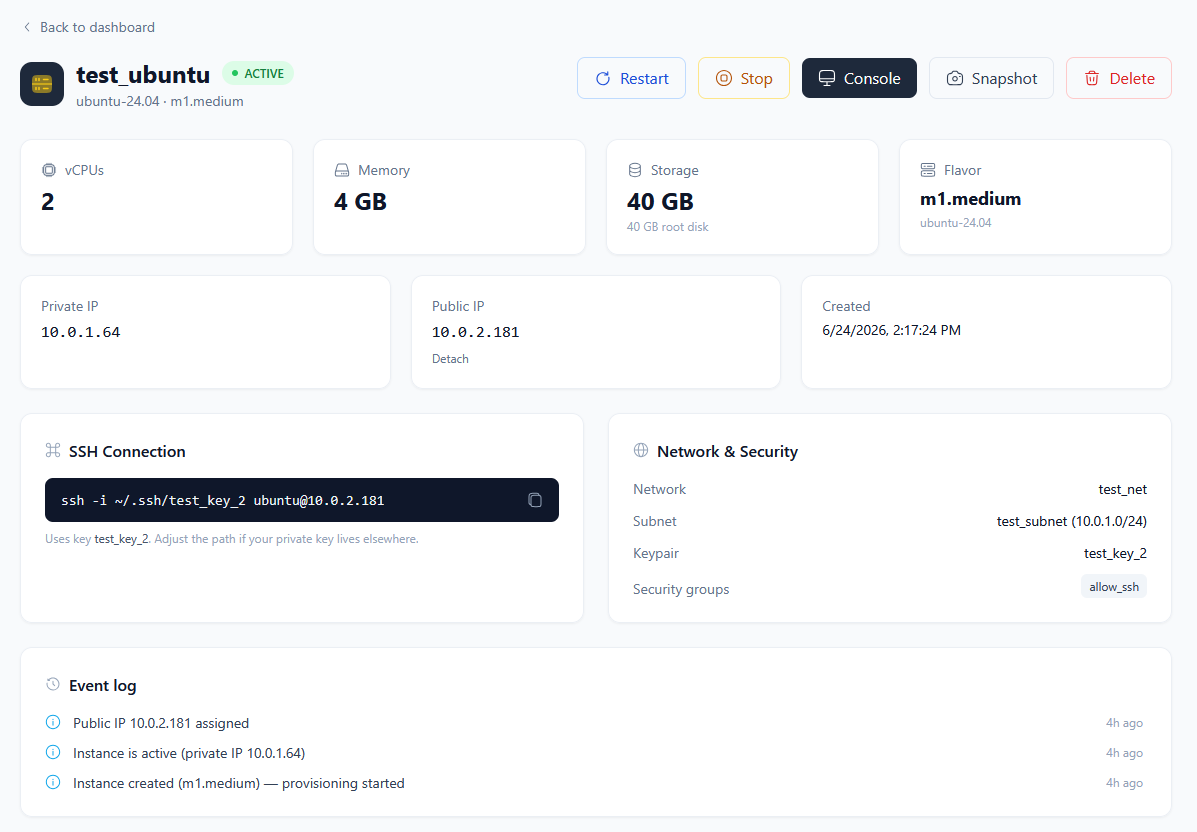
\includegraphics[width=0.8\textwidth]{continut/capitol4/figuri/instance_details.png}
    \caption{Provizionarea reușită a unei instanțe, verificată în platformă și în OpenStack.}
    \label{fig:cap4_dashboard}
\end{figure}

Pagina de detaliu din Figura~\ref{fig:cap4_dashboard} prezintă crearea cu succes a unei instanțe. Ea apare cu eticheta de stare \texttt{ACTIVE} și cu acțiunile disponibile asupra ciclului de viață (repornire, oprire, consolă, \textit{snapshot}, ștergere). Interfața arată resursele derivate din \textit{flavor}-ul ales (2 vCPU, 4 GB memorie, 40 GB stocare, \texttt{m1.medium}), iar secțiunea de adrese expune atât adresa IP privată alocată de Neutron, cât și adresa IP flotantă publică asociată automat. Panoul de rețea și securitate confirmă atașarea instanței la rețeaua și subrețeaua organizației, la perechea de chei și la grupul de securitate selectate. Comanda de conectare SSH este afișată, completată cu utilizatorul implicit și adresa IP. În partea de jos, \textit{jurnalul de evenimente} reconstituie cronologic întreaga provizionare, de la „instanță creată / provizionare inițiată”, la „instanță activă, adresă IP privată alocată” și „adresă IP publică asociată”.

\subsection{Verificarea cheii SSH}
\label{subsec:cap4_ssh}

Un criteriu crucial pentru o platformă VPS este ca utilizatorul să poată accesa mașina virtuală provizionată. Platforma generează perechea de chei pe server (cheia privată este returnată o singură dată și nu este niciodată stocată), încarcă cheia publică în OpenStack, iar Nova o injectează în instanță la prima pornire, prin mecanismul de \textit{metadata} utilizat de Cloud-init, care o scrie în fișierul \texttt{authorized\_keys} al utilizatorului implicit.

Verificarea a constat în conectarea reală prin SSH la o instanță provizionată, folosind cheia privată descărcată la generare și adresa IP flotantă asociată instanței (grupul de securitate permite traficul pe portul 22):

\begin{lstlisting}[basicstyle=\ttfamily\footnotesize,breaklines=true,frame=single]
# cheia privata salvata la generare; user implicit: cirros (sau ubuntu)
ssh -i cheie-privata.pem cirros@<adresa-IP-flotanta>
\end{lstlisting}

\noindent Conectarea reușește fără parolă, autentificarea fiind realizată exclusiv pe baza cheii. Acest rezultat validează întregul lanț al cheilor SSH: generarea criptografică în FastAPI, încărcarea în OpenStack de către procesul Celery, injectarea de către Nova la boot și utilizarea pentru acces.

\subsection{Accesul la consola noVNC}
\label{subsec:cap4_console}

Pe lângă accesul prin SSH (care presupune conexiune la rețea și o adresă IP publică), platforma oferă acces \textbf{în afara benzii} (\textit{out-of-band}) la consola grafică a mașinii virtuale, direct din browser. La solicitarea unei console, API-ul deleagă procesului Celery obținerea unui URL noVNC de la Nova, iar răspunsul este preluat sincron prin \textit{result backend}-ul Celery și deschis de interfață într-un cadru (\textit{iframe}). URL-ul indică proxy-ul noVNC al cluster-ului (\texttt{kolla\_internal\_vip\_address:6080}).

Verificarea a constat în deschiderea consolei din pagina de detaliu a unei instanțe active: consola grafică a mașinii virtuale s-a încărcat în browser, a afișat promptul de autentificare al sistemului de operare (Figura~\ref{fig:cap4_console}). Acest mecanism este de valoare în special atunci când accesul prin SSH nu este disponibil, de exemplu, înainte de asocierea unei adrese IP flotante sau în cazul unei configurări greșite a rețelei, oferind un canal de administrare independent de conexiunea la nivel de rețea a instanței.

\begin{figure}[H]
    \centering
    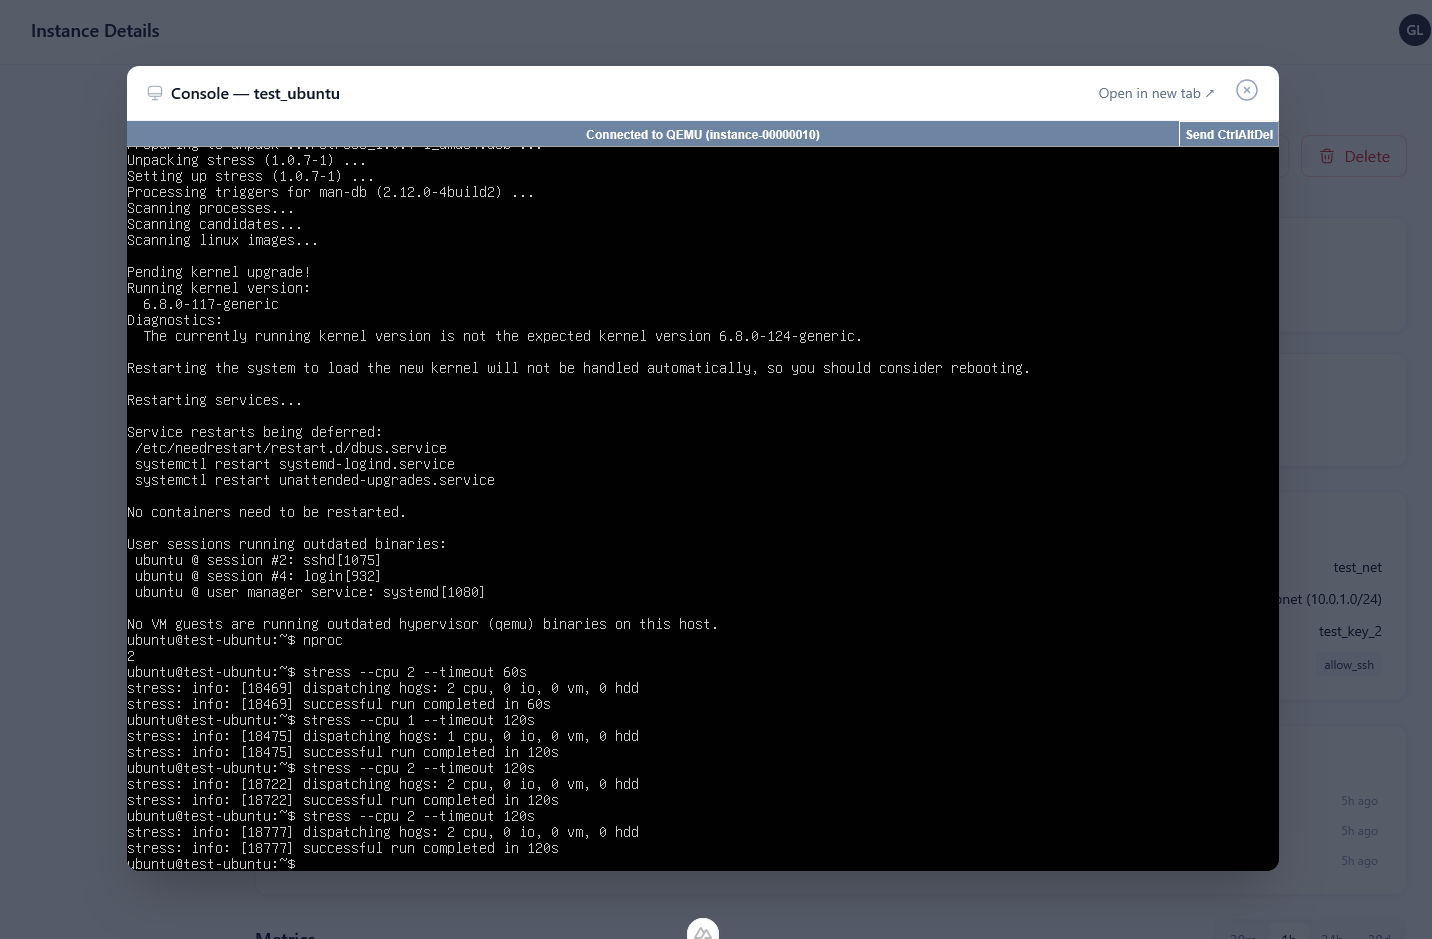
\includegraphics[width=0.8\textwidth]{continut/capitol4/figuri/noVNC.png}
    \caption{Accesul la consola grafică a unei instanțe prin noVNC.}
    \label{fig:cap4_console}
\end{figure}

Figura~\ref{fig:cap4_console} prezintă sesiunea noVNC încărcată într-o fereastră modală, direct în browser. Bara superioară confirmă o conexiune activă și criptată către instanță și oferă controale specifice unei console fizice: transmiterea combinației \texttt{Ctrl+Alt+Del} și deschiderea consolei într-o fereastră separată. Consola prezintă fluxul de ieșire al sistemului de operare: mesajele de pornire ale serviciilor, etapele de inițializare prin Cloud-init și promptul de autentificare al mașinii virtuale. Faptul că acest conținut este generat în timp real în interfață demonstrează că întregul canal funcționează, oferind un mijloc rapid de acces al instanței.

\subsection{Consola de administrare}
\label{subsec:cap4_admin}

Administratorul de platformă dispune de un panou care oferă o vedere de ansamblu asupra întregii platforme. Aceasta include capacitatea reală a cluster-ului OpenStack: numărul total de procesoare virtuale, memoria și spațiul de stocare, fiecare afișat ca valoare utilizată raportată la cea disponibilă, prin bare de utilizare, amprenta de resurse a fiecărei organizații și a fiecărui utilizator. Această perspectivă globală, prezentată în Figura~\ref{fig:cap4_admin}, permite monitorizarea consumului de resurse la nivelul întregii platforme și constituie suportul deciziilor de administrare, precum suspendarea organizațiilor sau ajustarea cotelor.

\begin{figure}[H]
    \centering
    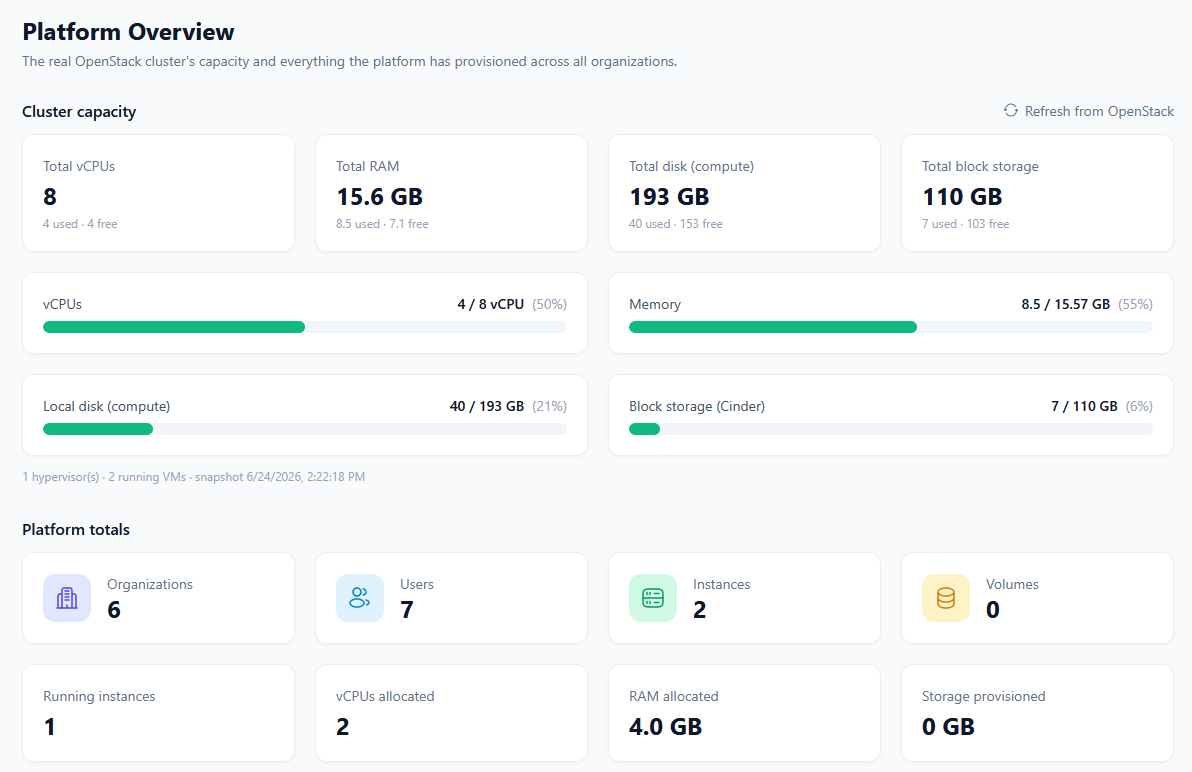
\includegraphics[width=0.85\textwidth]{continut/capitol4/figuri/admin_console.png}
    \caption{Consola de administrare, cu toate resursele utilizate la nivelul platformei.}
    \label{fig:cap4_admin}
\end{figure}

\subsection{Monitorizarea consumului de resurse}
\label{subsec:cap4_telemetrie}

Lanțul de telemetrie descris în Secțiunea~\ref{sec:cap3_telemetrie} a fost validat funcțional. Graficul de consum CPU din pagina de detaliu a unei instanțe (Figura~\ref{fig:cap4_cpu}) reflectă, pe baza datelor colectate periodic de procesul \textit{Celery Beat} și stocate în InfluxDB, evoluția în timp a utilizării procesorului. Pentru a confirma rezultatele graficului, s-a generat o încărcare controlată în interiorul unei instanțe (utilizând \texttt{stress-ng}), iar graficul a reflectat creșterea consumului, revenind ulterior la valori de repaus, în conformitate cu încărcarea reală a procesorului.

\begin{figure}[H]
    \centering
    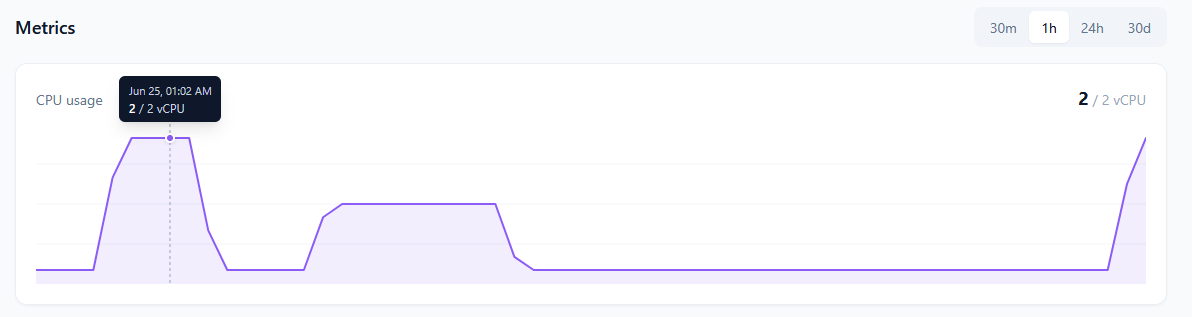
\includegraphics[width=0.85\textwidth]{continut/capitol4/figuri/metrics.png}
    \caption{Monitorizarea consumului de CPU al unei instanțe.}
    \label{fig:cap4_cpu}
\end{figure}

Figura~\ref{fig:cap4_cpu} prezintă graficul de monitorizare a consumului de CPU cu opțiunea de a selecta un interval temporal (30 de minute, 1 oră, 24 de ore, 30 de zile), ce permite ajustarea ferestrei de observație, iar valorile sunt raportate la numărul de procesoare virtuale alocate instanței (2 vCPU). Graficul evidențiază variația consumului în timp: intervale de repaus apropiate de zero, alternând cu vârfuri corespunzătoare perioadelor de încărcare, iar la trecerea cursorului peste grafic se afișează valoarea punctuală și momentul de timp asociat.

\section{Limitări}
\label{sec:cap4_limitari}

Etapa de testare a vizat și validarea comportamentului sistemului în condiții de excepție. În situația în care procesul de provizionare eșuează la nivelul serverului openstack, de exemplu la declanșarea erorii \texttt{NoValidHost} de către planificatorul Nova, din cauza epuizării resurselor de calcul, platforma nu rămâne într-o stare inconsistentă. Procesul de fundal Celery schimbă instanța în starea \texttt{ERROR}, înregistrează cauza eșecului în jurnalul de evenimente și inițiază un mecanism de reîncercare automată, limitat la un număr predefinit de iterații. Acest comportament atestă eficacitatea mecanismelor de reziliență proiectate. Rutina asincronă de reconciliere (\textit{Celery Beat}) verifică
la fiecare interval starea afișată cu starea reală raportată de Nova; astfel, orice schimbare apărută extern este reflectată în interfața utilizator.

Testarea a evidențiat totodată limitările mediului ales: 

\begin{itemize}
    \item \textbf{Nod unic, fără redundanță:} desfășurarea \textit{all-in-one} pe un singur nod nu oferă disponibilitate înaltă (\textit{High Availability}); o defecțiune a nodului afectează întreaga platformă.
    \item \textbf{Izolare logică, nu la nivel de infrastructură:} toate organizațiile împart un singur proiect OpenStack, izolarea fiind impusă la nivelul aplicației prin filtrare după organizație; o izolare strictă ar necesita un proiect OpenStack per organizație.
    \item \textbf{Procesare serială pe Windows:} pe sistemul de dezvoltare, procesul Celery rulează cu opțiunea \texttt{--pool=solo}, ceea ce serializează execuția sarcinilor; pe Linux, cu un \textit{pool} de procese, sarcinile s-ar executa concurent.
    \item \textbf{Stocare partajată și limitată:} pe un nod unic, volumele Cinder (backend LVM peste un fișier \textit{loopback}) și discurile efemere ale instanțelor Nova sunt pe același disc fizic al mașinii, fără un sistem de stocare dedicat sau distribuit. Capacitatea totală și performanța de I/O sunt astfel partajate între calcul și stocare, iar volumul disponibil pentru instanțe este limitat de discul unic.
    \item \textbf{Virtualizare imbricată:} cluster-ul OpenStack rulează el însuși într-o mașină virtuală (VMware), astfel încât hypervisor-ul Nova (KVM) operează în regim de \textit{nested virtualization}. Acest strat suplimentar introduce o penalizare de performanță față de execuția pe hardware nativ și limitează capacitatea reală de calcul.
    \item \textbf{Adrese IP „publice” doar în rețeaua de laborator:} adresele IP flotante provin dintr-un bazin extern definit în mediul de testare, accesibil de la distanță exclusiv prin tunelul Tailscale, nu din internetul public. Într-un mediu de producție ar fi necesar un bazin de adrese rutabile real.
\end{itemize}

